During the past decade, the amount of data in the world has grown at exponential rates and is currently showing no signs of slowing down. According to infographics released by IBM, already 2.7 ZB\footnote{Zettabytes. 1 Zb = 1 trillion Gb.} of data existed in the world in 2012 \cite{karr_2012}, enough to fill up almost 40 billion 64 Gb iPhones. This number has since then risen to 8 Zb in 2015 and is expected to reach a yearly production of 35 Zb by 2020 \cite{deutscher_2012} \cite{karr_2012}. 85\% of all the world data is considered to be unstructured data \cite{blumberg2003problem}, which is mainly be made up of multimedia in the form of images and videos. An important factor in this growth is the rise of mobile devices usage and social media. Indeed, the amount of mobile-dependant users has grown at impressive rates, with now 95\% of the United States citizens owning a mobile phone \cite{fanning2012increasing}. People tend to use their mobile devices for most day-to-day activities, with a majority of this time spent on social media services such as YouTube or Facebook. The social networks are one of the primary causes for the exponential growth of unstructured data mentioned earlier, with over 300 hours of new video content is uploaded to YouTube every minute of the day. The combination of mobile devices usage and social media data are the main contributors in today's flood of unstructured data. This project will look at creating a system combining the problem of unstructured data in the form of video data on mobile devices.

\section{Problem Description}
\label{sec:problem-description}

Content-based video retrieval is a computer vision solution to the problem of searching large databases of videos, where "content" corresponds to information from the videos such as colours or shapes that can be used to efficiently retrieve a desired video from the database. The main difficulty with content-based video retrieval lies with the reference database of videos itself. Videos in a database correspond to unstructured data, meaning only the video data\footnote{Video data includes the video frames and the audio.} and their metadata\footnote{Examples of metadata related to a video file includes captions, file name, file type, video length, file size, etc.} are stored in the database. Computations involved in querying a database of videos using only the metadata available without the ability to analyse the video files would be too expensive and highly inefficient \cite{patel2012}. Therefore, the inspection of the video files is a necessity to find solutions to the database complication in content-based video retrieval. It is important to note that the metadata can still be used as a complement to the video files analysis to fine-tune the pattern matching. Another complication involves the large database size. Indeed, more complications arise from databases populated with a large number of videos, especially if their duration is lengthy e.g. feature-length films. Solutions to those problems hence require intelligent and efficient pattern matching algorithms to overcome the specified difficulties. This is where visual search and the variety of fields it includes such as artificial intelligence, machine learning and database management come in.\\

Several visual search techniques exist for querying databases of unstructured data such as video or image files. These techniques can be classified based on the type of query and on the type of database used, as shown in table \ref{table:visual_search_table}. The most common forms of visual search consist in querying a database of images either with an image (I2I) or with a video (V2I), as depicted in section \ref{sec:v2v_applications} where similar existing systems are mentioned. Another less frequent variant consists of querying a database of images with a video query (V2I) \cite{araujo2017i2v}. However, this dissertation will solely focus on querying a database of videos with a video query (V2V). Because algorithms from other variants of visual search can be relevant to V2V, existing solutions for these variants will also be explored to find ways potential techniques that could be implemented with this project.\\

% types of visual search table
\begin{table}[H]
\centering
\begin{tabular}{c|c|c|}
\hline
\multicolumn{1}{|c|}{Image Query} & I2I                & I2V                \\ \hline
\multicolumn{1}{|c|}{Video Query} & V2I                & V2V                \\ \hline
\multicolumn{1}{l|}{}             & Database of Images & Database of Videos \\ \cline{2-3} 
\end{tabular}
\caption{The four types of visual search involving images and videos, classified by type of query used and by type of database being queried.}
\label{table:visual_search_table}
\end{table}

To pattern match the query video to a video in the database, key elements from the query video, called \textit{"features"}, are extracted and compared to the same features from videos in the database to find similarities. These features can include elements such as colour histograms or shapes of interest and their on-screen movements \cite{patel2012}, as well colour percentages, colour layouts or textures \cite{petkovic2000}, or other unique features such as on-screen text or audio components e.g. soundtracks, dialogues or sound effects. A wide spectrum of existing solutions exists to efficiently retrieve videos using video queries, which are discussed in the section below.

\section{Related Content-Based Retrieval Systems and Their Applications}
\label{sec:v2v_applications}

Visual search technology has an endless amount of applications in fields such as education, navigation, utilities and security. Some of the systems using this technology have already found their way to commercial applications. For example, YouTube's Content ID system uses visual search, and more precisely V2V, to detect copyright infringements on user-uploaded videos by automatically comparing an uploaded video with a database of protected videos provided by their partners. If a match is found, YouTube allows these partners to take action on the uploaded video that infringed their copyrights \cite{youtube-content-id-2012}. Another example is Google Lens \cite{google-lens}, a mobile application that recognises the input context through a mobile device's camera in order to relay information about objects of interest. For instance, if pointing the camera at a landmark, information such as historical facts or opening hours about that location will be displayed, or if pointing it at a WiFi router's label, the mobile device will automatically connect to the network \cite{villaboas-google-lens2017}. Other profitable applications include A9's Amazon Flow \cite{a9-visual-search} that uses deep-learning based computer vision for Amazon's search services, as well as Shazam \cite{shazam}, a mobile application that matches short user-recorded sounds with a piece of music.\\

Aside from the commercialised systems stated in the previous paragraph, many visual search applications are yet to be implemented for large-scale use. For example, a system allowing companies to detect all appearances of their logos during television broadcasts, or a system enabling students to find a section of a recorded lecture by using a lecture slide as a query \cite{araujo2017i2v} are possibilities that need to be explored. Content-based video retrieval academic papers have also been published in recent years. For instance, Liu et al. \cite{liu2014mobilevideosearch} discuss a concept similar to this project's idea consisting of a mobile visual search system allowing users to discover videos by pointing their phone at a screen. Recently, research in visual search has gained momentum, notably with the annual TRECVID\footnote{Text REtrieval Conference Video Retrieval Evaluation} conference \cite{2018trecvidawad} hosted by the NIST\footnote{National Institute of Standards and Technology}. This conference's goal is to host workshops that focus on information retrieval research, with an emphasis on content-based retrieval of digital videos \cite{trecvid-general}. The combination of academic research and specialised conferences will hopefully help bring more content-based retrieval solutions to real-life problems.

\section{Project Aim}

This project aims to find solutions to address the previously mentioned problems from Section \ref{sec:problem-description}, namely:

\begin{itemize}
    \item the exponential rise of unstructured data in the form of media, with a focus on videos,
    \item the over-reliance people have on their mobile devices for basic day-to-day tasks,
    \item the sparse collection of existing solutions that could be combined to create more efficient systems,
    \item the lack of focus on videos, especially feature-length movies.
\end{itemize}

This project will attempt to translate solutions to the mentioned problems by creating a system that will combine existing solutions into a single one, with a focus on recognising a feature-length movie from a short video query recorded from a mobile device, as depicted in Figure \ref{fig:wireframe}.

\begin{figure}[h]
\centerline{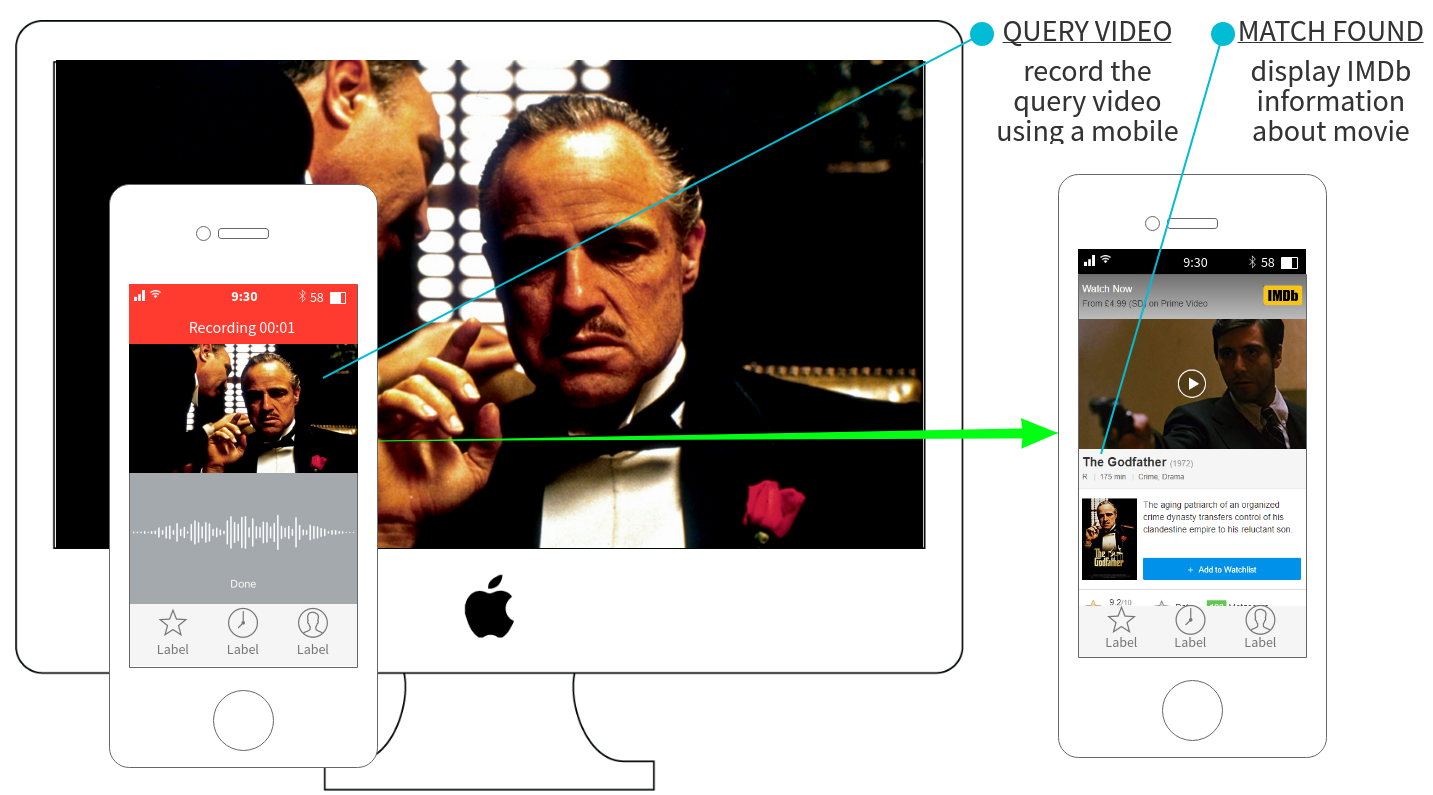
\includegraphics[width=1.15\textwidth]{figures/introduction/system_wireframe.png}}
\caption{\label{fig:wireframe}Wireframe showing the basic high-level concept that the system will try to achieve.}
\end{figure}

\section{Project Structure}

This project adopts the following structure:

\begin{enumerate}
    \item Chapter 1: Introduction
    \item Chapter 2: Literature \& Technology Survey
    \item Chapter 3: Requirements
    \item Chapter 4: Design
    \item Chapter 5: Implementation
    \item Chapter 6: System Testing
    \item Chapter 7: Evaluation
    \item Chapter 8: Discussion
    \item Chapter 9: Conclusion
    \item Appendix XXX: 13 Point Ethics Check List
    \item Appendix XXX: Experiment Survey
    \item Appendix XXX: Raw Experiment Results
\end{enumerate}
